%!TEX root = main.tex
\section{Study Findings}
\subsection{Themes Emerging from Participatory Design\label{pd_findings}}
\begin{figure*}[ht!]
\centering
\vspace{-15pt}
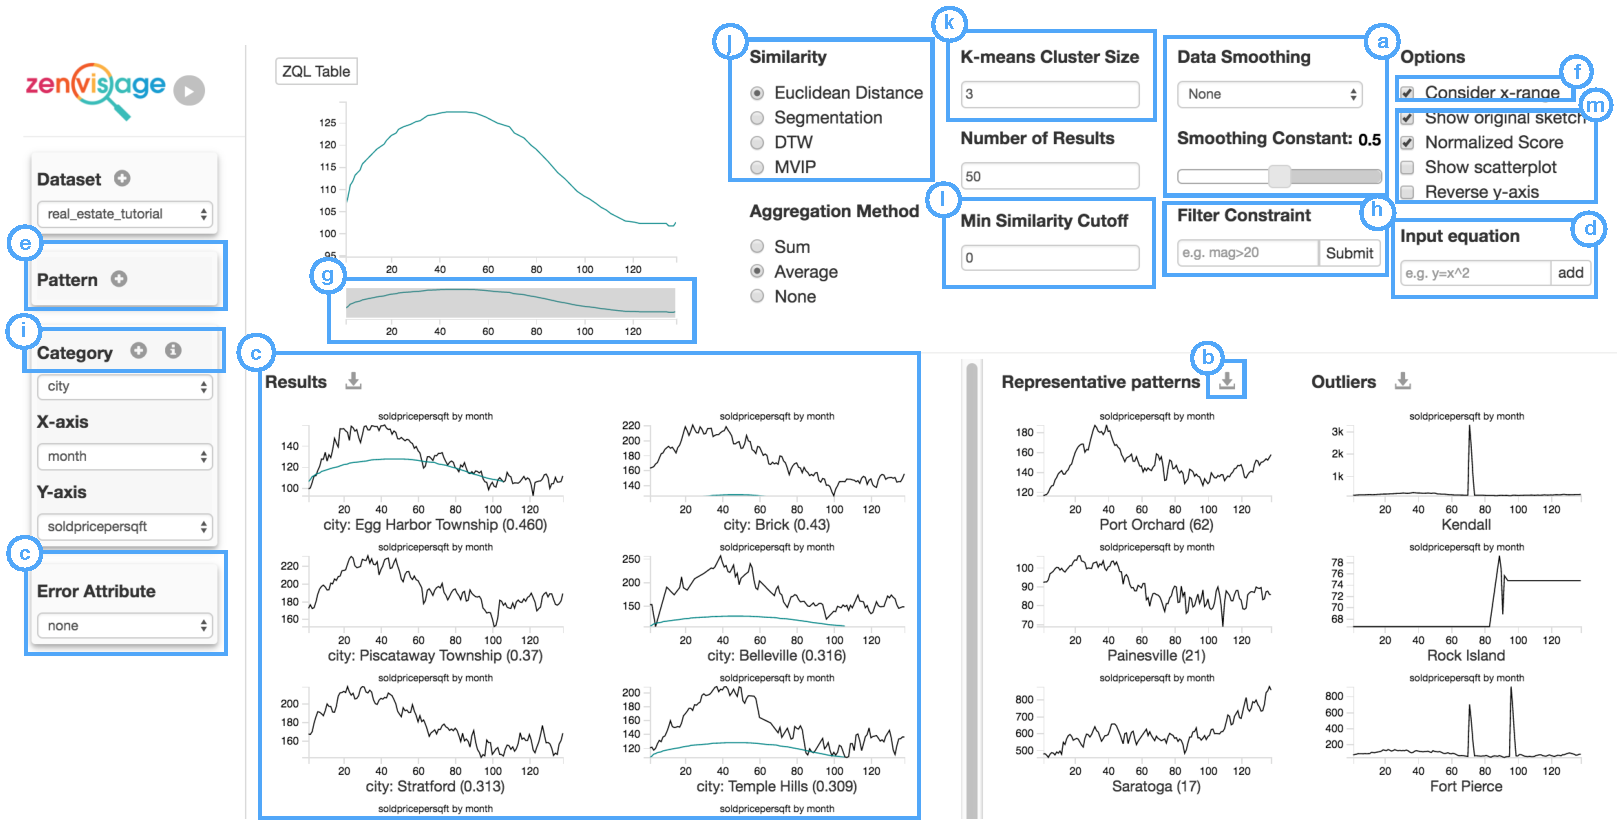
\includegraphics[width=\linewidth]{figures/newZV.pdf} %5.5
\vspace{-5pt}\caption{Our VQS after participatory design, which includes: the ability to preprocess via (a) interactive smoothing; (b, c) the ability to export data outputs ; querying functionalities via (d) equations and (e) patterns; query specification mechanisms including (f) x-range invariance, (g) x-range selection and filtering, (h) Filtering, and (i) Dynamic class creation; (j, k, l) system parameter options; (m) visualization display options. Prior to the participatory design, \zv only included a single sketch input with no additional options.}
\label{zvOverview}
\vspace{-14pt}
\end{figure*}

\par We employed participatory design with our scientists to incorporate key features missing in our original VQS, and unaddressed in their existing workflows. %We discovered three central themes encapsulating these features that are important to facilitate rapid hypothesis generation and insight discovery, but are missing in prior VQSs. While some of our findings echo prior work on system-level taxonomies of visualization tasks \cite{Amar2005,Heer2012}, we highlight how specific analytic tasks and interaction features could be used to enhance VQSs in particular. \techreport{In particular, we learned that \textit{participants wanted more control over the internals of the systems and an integrated workflow that helped streamline their analysis when using VQSs.}}
\boldpara{Exact Shape Specification}
Exact shape specification interfaces allows users to submit a query through an exact description of a pattern, then the VQS returns a list of most similar matches. Almost all VQS supports freehand sketching on a virtual canvas through mouse or pen as a intuitive mechanism for specifying a desired patterns. In addition to sketching, \zv also allows users to specify a functional form for a sketchWe implemented a feature that plots a given function (e.g. $y=x^2$) on the canvas, which is then used as input for similarity search (Figure \ref{zvOverview}d). This feature was inspired by material scientists who were interested in finding solvents with known analytical models that characterize the relationships between their chemical properties.
\boldpara{Approximate Shape Specification}
While exact shape specification is an intuitive mechanism for constructing a visual query, a pattern query can be extremely imprecise, as pointed out by past works~\cite{correll2016semantics,Holz2009}. Many interfaces have developed constrained sketching mechanism to allow users to partially specify certain characteristics of a pattern, while leaving the rest to convey the intent of an inexact match, such as angular slope queries for specifying the slope of a trend line~\cite{Hochheiser2004} or piecewise trend querylines over a specified data range~\cite{ryall2005querylines}. Both Qetch~\cite{Mannino2018} and \zv supports data smoothing to allow users to interactively change the degree of shape approximation they would like to apply to all visualizations (and consequently for pattern matching). We develop an interface for users to interactively adjust data smoothing algorithm and parameters on-the-fly to update the resulting visualizations accordingly (Figure \ref{zvOverview}a).
\par During participatory design, both material science and astronomy participants noted the difficulty of shape matching on their dense and noisy observational data and the challenge of picking the appropriate smoothing parameters during offline preprocessing. We found that the tight integration between smoothing and visual search additionally poses an interesting relationship between the smoothness of the curve and the degree of approximation for shape-matching in VQSs. If the visualization is over-smoothed, then shape matching would return results that only loosely resemble the query pattern. However, if no smoothing is applied, then the noise may dominate the overall trend, which could also lead to bad pattern matches.
%While the interactions in our original prototype enabled simple visual queries, many scientists were interested in extending their querying capabilities, either through different querying modalities or through more flexible query specification methods.

% While \zv does not attempt to solve all of the pre-processing issues that we faced during participatory design, we identified data smoothing as a common data cleaning procedure that could benefit from a tight integration between pre-processing and visual analysis. Data smoothing is a denoising procedure that generates a smoothed pattern approximating key features of the visualized trend with less noise.
\boldpara{Range Selection}
One common additional specification on top of the exact or approximate shape query is limiting the pattern query matched to specific x or y ranges. time series analysis where measure range and time range has special domain specific significance. Range selection can be performed through explicit specification through textbox entry~\cite{wattenberg2001sketching,Mannino2018}, drawing line limits~\cite{ryall2005querylines}, or brushing interactions~\cite{Hochheiser2001}. \zv employs the brushing mechanism to select desirable x-ranges to perform shape matching (Figure \ref{zvOverview}g), additionally, y axis range selection could be performed through entering a filter constraint on the measure variable.
\par We chose to support only brushing for x, since it was more common to focus the context based on the independent variable in the use cases, such as zooming into particular sharp dips when looking for planetary transits or anomalous peaks indicative of erroneous experimental measurements. In contrast, y-range selection tends to be more global and enforced across multiple interaction sequences, such as looking for only signals above a certain threshold. The TimeSearcher and Queryline approach is most flexible for range selection as they allow composition of multiple range selection to formulate complex piecewise queries, such as a gene expression profile rising from x=1$\sim$5 and declining from x=5$\sim$10.
\boldpara{Flexible Matching}
Studies have shown that to facilitate subjectively meaningful pattern matches, VQSs need to support mechanisms for clarifying sketch interpretation and flexible shape matching algorithms~\cite{correll2016semantics,Mannino2018,Eichmann2015}. \zv offers selection tools allowing users to change similarity metrics that perform flexible matching, such as DTW, MVIP, and segmentation. In addition, we give user the option to ignore the x-range in shape matching (Figure \ref{zvOverview}f). For finding supernovae, A1 primarily cared about the existence of a peak above a certain amplitude with an appropriate width of the curve, rather than the exact time that the event occurred, leading them to use the consider x-range feature. G1 also expressed that she does not really know what is the ``trigger point'' of when the expression level of a gene will rise and it would be interesting to find all ``rising'' profiles independent of the change-point. These features are akin to the temporal invariants in SketchQuery~\cite{correll2016semantics}.

\boldpara{Filter Selection}
\par Past studies in taxonomies of visualization tasks have shown that it is important to design features that enable users to select relevant subsets of data in visual analytics\cite{Amar2005,Heer2012}. %We designed two dynamic faceting features coupled with coordinated views that enabled users to specify subsets of data they are querying on and see immediate changes updated in the query, representative, and outlier results.
We find that users with large datasets first used their domain knowledge to narrow down their search to a subset of data. This would increase their chances of finding an interesting pattern for a given pattern query. To filter data, users could compose one or more SQL-like \texttt{WHERE} conditions as filter constraints in a text field (Figure \ref{zvOverview}h). The filtering can be done on data columns associated with each pattern that is not visualized or on the visualized attributes. This feature is unique to \zv as most existing VQSs do not allow users to interact with data in the non-visualized columns.
\boldpara{Group Comparison}
A common analytical question from our participatory design is that users often want to bucket data points into customized classes based on existing properties, and subsequently compare between the customized classes. For example, material scientist M1 wanted to create classes of solvents with ionization potential under -10 kJ/mol, over -8 kJ/mol, and ones that fall between -10 and -8 kJ/mol. Then, he could browse how visualizations involving lithium solvation energy varied across the three classes. To this end, we implemented dynamic class creation, a feature that allows users to use multiple properties to create custom classes on-the-fly, effectively slicing-and-dicing the data based on their needs. The information regarding the created classes is displayed in the dynamic class information table and as a tooltip over the aggregated visualizations, as shown in Figure~\ref{dcc}.
\begin{figure}[h!]
\centering
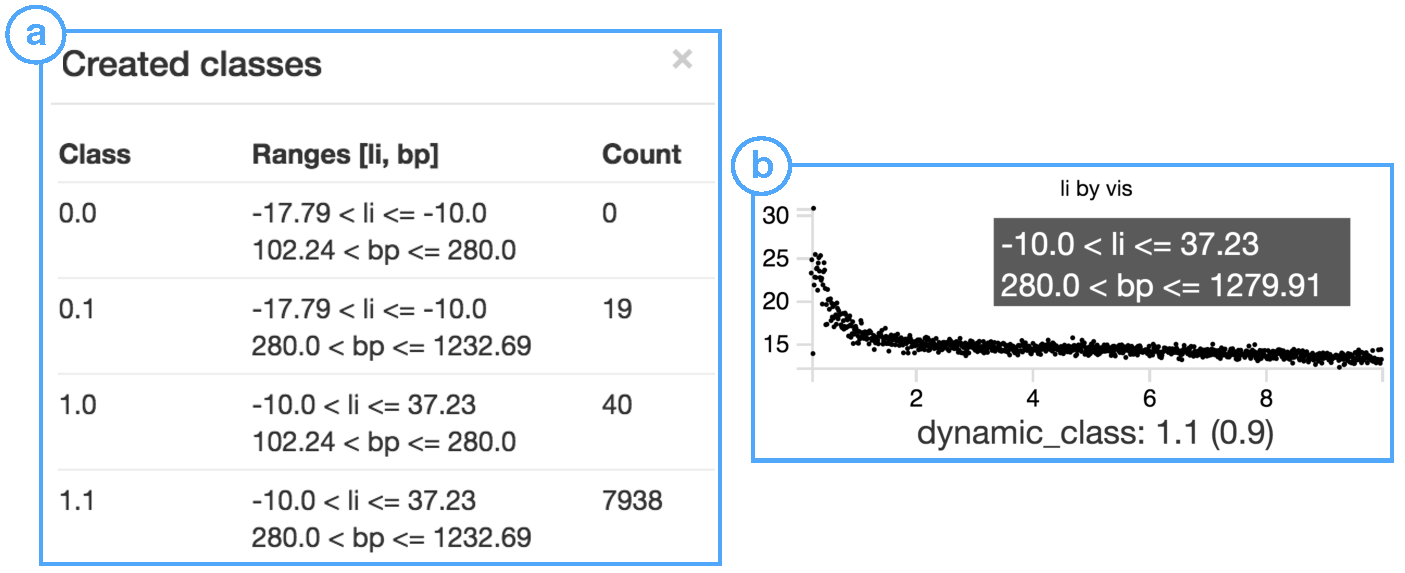
\includegraphics[width=\linewidth]{figures/dcc_example.pdf}
\vspace{-6pt}
\caption{Example of dynamic classes. (a) Four different classes with different Lithium solvation energies (li) and boiling point (bp) attributes based on user-defined data ranges. (b) Users can hover over the visualizations for each dynamic class to see the corresponding attribute ranges for each class. The visualizations of dynamic classes are aggregate across all the visualizations that lie in that class based on the user-selected aggregation method.}
\label{dcc}
\vspace{-10pt}
\end{figure}
\boldpara{Concept querying}
While the input equation is useful when simple analytical models exist, this may not be true for other domains. In these cases, users can upload a query pattern of a sequence of points (Figure \ref{zvOverview}e). This is useful for patterns generated from advanced computational models used for understanding scientific processes or prelabelled data from an external reference database. For example, astronomer A1 can upload a query pattern based on synthetic light curves generated from simulations~\cite{Nugent1997} or known supernovae that have been discovered in the past.
%, usually as part of the downstream analysis of the exploratory workflow. %For example, the genetics team are trying to develop a time series prediction algorithm using machine learning based on some biological parameters \cite{Peng2016}.
\boldpara{Result-based querying}
TimeSearcher allows users instantiate timebox queries by dragging a result visualization and dropping into the query space; QuerySketch does so similarly through double clicking on the visualization. Similarly in \zv, users can drag and drop a visualization in either the results pane or the representative and outliers.
\boldpara{Recommendation}
\zv provides visualization recommendations ---- representative and outliers

\subsection{Evaluation Study Results\label{eval_findings}}
We recorded audio, video screen captures, and click-stream logs of the participant's actions during the evaluation study. We analyzed the transcriptions of these recordings through open-coding and categorized every event in the user study. In addition, based on how each feature was used during the user study, we categorized the features into one of the three usage types:
\begin{denselist}
    \item Practical usage \textbf{[P]}: Features used in a sensible and meaningful way.
    \item Envisioned usage \textbf{[E]}: Features which could be used practically if the envisioned data was available or if they conducted downstream analysis, but was not performed due to the limited time during the user study.
    \item Not useful \textbf{[N]}: Features that are not useful or do not make sense for the participant's research question and dataset.
\end{denselist}
We chose to derive these labels from the user study transcription rather than through self-reporting to circumvent the bias that users may have when self-reporting, which can often artificially inflate the usefulness of the feature or tool under examination.
\begin{figure}[ht!]
    \centering
    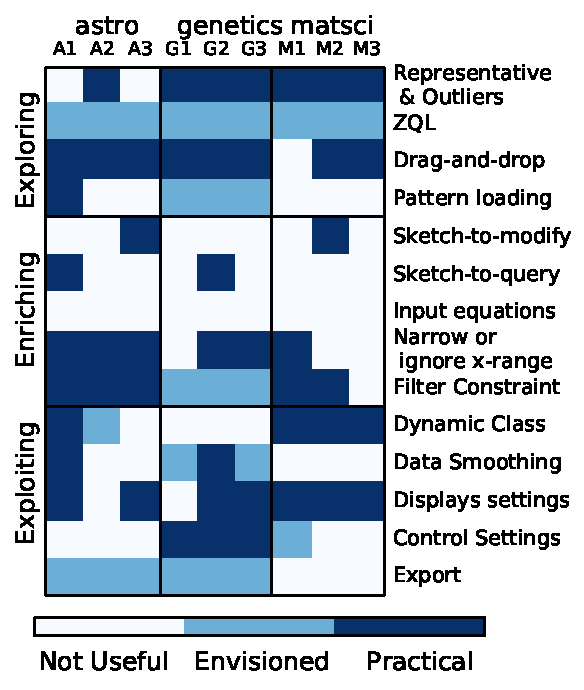
\includegraphics[width=0.7\columnwidth]{figures/result2.pdf}
    \vspace{-6pt}\caption{Heatmap of features categorized as practical usage (P), envisioned usage (E), and not useful (N). We find that participants preferred to query using bottom-up methods such as drag-and-drop over top-down approaches such as sketching or input equations. Participants found that data faceting via filter constraints and dynamic class creation were powerful ways to compare between subgroups or filtered subsets. The columns are arranged in the order of subject areas and the features are arranged in the order of the three foraging acts.}
    \label{feature_heatmap}
    \vspace{-5pt}
\end{figure}

\par The audio recordings and transcriptions of pre- and post-study interview questions are thematically encoded and summarized in Figure \ref{action_heatmap} and \ref{feature_heatmap}. Overall, we find that VQSs can enable rapid, fluid iteration, catalyzing new questions or insights; that different querying modalities in VQSs support different forms of exploration; and that expressive querying allowed participants to compose novel analysis patterns. In addition, we find that VQSs can be used for a range of tasks that go beyond just exploration; that participants used the outputs from VQSs in various ways; and that VQSs are most appropriate for certain types of datasets.
For the remaining paper, we will focus on developing a process model and design guideline for insight formation in VQSs and divert our thematic analysis of how VQSs fit into the context of an analysis workflow to our technical report.

% These observation inform our ----- search-browse paradigm
